\documentclass[doktyp=barbeit, sprache=german]{TUBAFarbeiten}
\usepackage[utf8]{inputenc}
\usepackage[T1]{fontenc}
\usepackage{graphicx} 
\usepackage{amsmath}
\usepackage{subcaption}
\usepackage[Algorithmus]{algorithm}
\usepackage{algorithmicx}
\usepackage[noend]{algpseudocode}
\usepackage[numbers]{natbib}
\usepackage{booktabs}
\usepackage{rotating}
\usepackage{lscape}
\usepackage{mwe}
\usepackage{listings}
\usepackage{xcolor}

\newcommand*\rfrac[2]{{}^{#1}\!/_{#2}}

\lstset { %
    language=C++,
    backgroundcolor=\color{black!5}, % set backgroundcolor
    basicstyle=\footnotesize,% basic font setting
    numbers=left
}



\captionsetup{compatibility=false}
\bibliographystyle{unsrt}
\TUBAFFakultaet{Fakultät für Mathematik und Informatik}
\TUBAFInstitut{Institut für Informatik}
\TUBAFLehrstuhl{Lehrstuhl für Künstliche Intelligenz und Datenbanken}
\TUBAFTitel{Eine Studie zur kombinatorischen Optimierung mit Ameisenalgorithmen}
\TUBAFBetreuer{Prof. Dr. H. Jasper}
\TUBAFKorrektor{M. Sc. V. Göhler}
\TUBAFAutor[S. Dressel]{Samuel Dressel}
\TUBAFStudiengang{Angewandte Informatik}
\TUBAFVertiefung{Künstliche Intelligenz}
\TUBAFMatrikel{59\,963}
\TUBAFDatum[2018-11-05]{05. November 2018}
\begin{document}
\maketitle
\tableofcontents
\newpage
\section{Einleitung}
\section{Grundlagen}
\subsection{Der Ameisenalgorithmus (Ant Colony Optimization)}
\subsubsection{Biologische Grundlagen}
Für das weitere Verständnis des \textit{Ameisenalgorithmus} (auch Ant Colony Optimization Algorithm oder kurz ACO) ist zunächst ein Blick auf die biologischen Grundlagen notwendig. Ein Tierstaat, wie er bei den Ameisen zu finden ist, funktioniert nur mit einer effektiven und sinnvollen Kommunikation. Methoden zur Verständigung wie das Kommunizieren über Vibrationen und Berührungen sind eher die Ausnahme und kommen nur in speziellen Situationen zum Tragen \cite{Ameisen}. Dagegen kommt zum größten Teil der Informationsaustausch über Duftstoffe (sog. Pheromone) zur Anwendung. Diese werden durch verschiedene Drüsen erzeugt und wiederum in unterschiedlicher Kombination und Konzentration abgegeben.
Diese Pheromone werden benutzt, um Nestgenossen zu erkennen oder um bei Gefahren Kampf- und Abwehrverhalten auszulösen. Hauptsächlich jedoch nutzen Ameisen die Pheromone um eine Duftspur über ihren Hinterleib abzugeben. Diese dient ihnen und dem restlichen Tierstaat als Orientierungshilfe. Zum einen werden damit Straßen zu anderen Kolonien gebildet - zum anderen dienen sie dazu, anderen Ameisen den Weg zu einer Nahrungsquelle zu zeigen. Die Tatsache, dass ein Weg mit einer höheren Pheromonkonzentration bevorzugt wird, ist Grundlagen des Ameisenalgorithmus.
\subsubsection{Der Ameisenalgorithmus}
Der historische Ursprung des Algorithmus findet sich in den Versuchen von Jean-Louis Deneubourg und seine Kollegen \cite{Biological}. Das sogenannte \glqq Double-Bridge-Experiment\grqq \,zeigte, dass Ameisen den kürzesten Weg aufgrund der Pheromonmarkierung finden. In diesem Experiment ist eine Kolonie von Argentinischen Ameisen mit einer Nahrungsquelle durch zwei Brücken verbunden, die gleichzeitig den einzigen Zugang zu dieser Nahrungsquelle bilden. \cite{Dorigo2007}. Dabei können die Ameisen die Futterquelle nur über diese zwei Brücken erreichen. Im ersten Teil des Versuchs sind diese beiden Brücken jeweils gleich lang (siehe Abbildung \ref{img:DBExperiment}a). Zu Beginn erkunden die Ameisen die Umgebung der Kolonie bis sie eine Entscheidung über die Auswahl der Brücke treffen müssen. Lässt sich aufgrund einer noch nicht stattgefundenen Begehung der Brücken keine Pheromonspur feststellen, so entscheiden die Ameisen rein zufällig welche Brücke sie wählen. Die Wahrscheinlichkeit für beide Wege liegt bei gleichen Bedingungen bei 50 Prozent. Wird der Versuch über längere Zeit durchgeführt, so wird durch Zufall die Pheromonkonzentration der einen Brücke höher sein als die der anderen. Diese wird dadurch attraktiver für die Ameisen und wird somit letztenendes der favorisierte Weg zur Nahrungsquelle. 
\\Im zweiten durchgeführten Versuch sind die beiden Brücken unterschiedlich lang (siehe Abbildung \ref{img:DBExperiment}b). Auch hier liegt die Wahrscheinlichkeit für beide Brücken zu Anfang bei 50 Prozent. Da die Ameisen, die sich für die kürzere Brücke entscheiden, schneller wieder zurück am Nest sind, steigt das Pheromonlevel auf diesem Weg deutlich schneller an. Nach einiger Zeit kristalliert sich die kürzere Brücke als optimale Route heraus, während der längere Weg durch eine natürliche Pheromonverdunstung immer unattraktiver wird. Im Vergleich zum ersten Versuch geschieht der Ausbau der Pheromonspur wesentlich schneller und effektiver.
\begin{figure}
\captionsetup[subfigure]{justification=centering}
\centering
\begin{subfigure}[c]{0.45\textwidth}

\includegraphics[width=0.9\textwidth]{images/RouteTrivial.png}
\subcaption{Skizze zu Versuch 1; beide Wege sind gleich lang}
\end{subfigure}
\begin{subfigure}[c]{0.45\textwidth}
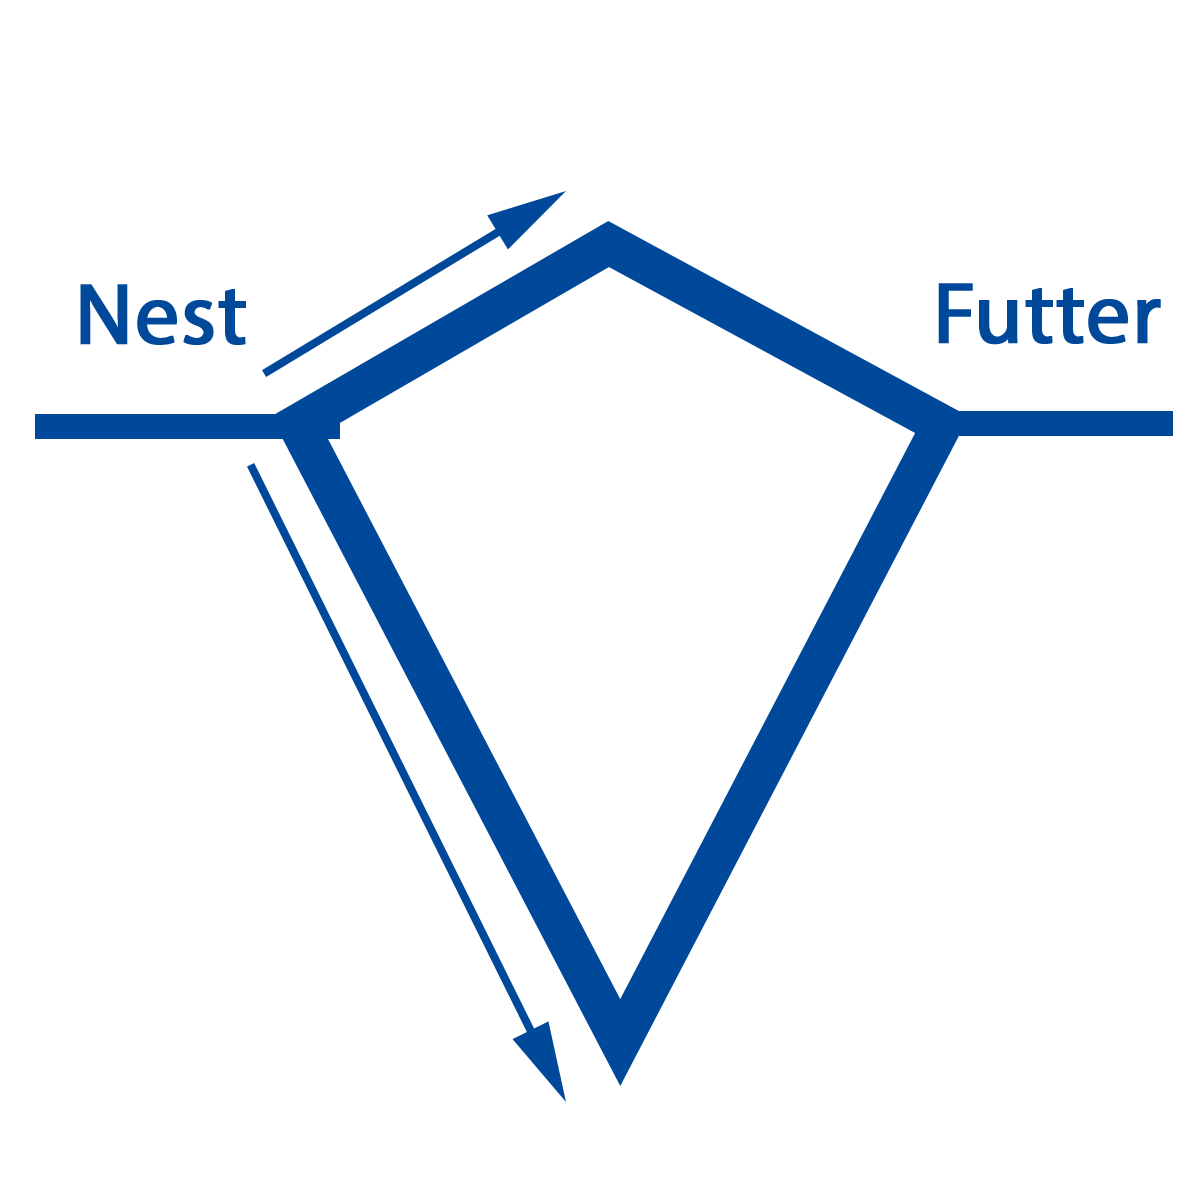
\includegraphics[width=0.9\textwidth]{images/RouteAdv.png}
\subcaption{Skizze zu Versuch 2; die Wege sind unterschiedlich lang}
\end{subfigure}
\caption{Double-Bridge-Experiment nach Deneubourg \cite{Biological}}
\label{img:DBExperiment}
\end{figure}
\subsection{Das Travelling-Salesman-Problem}
\subsubsection{Das Problem im Allgemeinen}
Das \textit{Travelling Salesman Problem} (im Folgenden mit TSP abgekürzt) ist eines der bekanntesten und meist untersuchten Optimierungsprobleme \cite{TaschenbuchAlgorithmen}. Kerninhalt des Problems ist dabei folgender: Ein Handlungsreisender soll in einer Rundreise \(n\) verschiedene Städte besuchen. Der Reisende startet dabei (zufällig) in einer dieser Städte und am Ende seiner Reise kehrt er auch wieder in diese Stadt zurück. Dabei sollen alle $n$ Städte nur einmal besucht werden und die Weglängen bzw. die Kosten der gesamten Reise minimal sein.
\\Seinen geschichtlichen Ursprung hat das TSP im Jahr 1832, als in Deutschland ein Buch mit dem Titel \glqq Der Handlungsreisende, wie er sein soll und was er zu thun hat, um Aufträge zu erhalten und eines glücklichen Erfolges in seinen Geschäften gewiss zu sein\grqq erschien. Dieses Buch und dessen Inhalt diente als Grundlage für die Erforschung des Problems. Die erste Benutzung des Ausdrucks \glqq Traveling Salesman Problem\grqq erfolgte in mathematischen Kreisen etwa um das Jahr 1931 \cite{TSP}. 
Dies geschah als mehrere amerikanische Mathematiker sich des Problems annahmen - wichtige Vertreter waren dabei Merrill Flood und Hassler Whitney, die die Überlegungen des österreichischen Mathematikers Karl Menger als Grundlage nahmen. Nach und nach wurde das Problem durch zahlreiche Veröffentlichungen immer präsenter und bis heute ist das TSP eines der prominentesten und am besten untersuchten Probleme in der Mathematik.
\subsubsection{Graphentheoretische Grundlagen} \label{graphbasics}
Um das Problem formal als ein graphentheoretisches Problem darzustellen, werden im Folgenden die dafür benötigten Begriffe definiert \cite{graphKemnitz}:
\\\\$G = (V,E,c)$ sei zunächst ein \textit{ungerichteter Graph}. Dabei beschreibt $V = \{1,...,n\}$ die Menge der Knoten und $E$ die Menge der Kanten, welche letztenendes eine Menge von ungeordneten Paaren $e \in E = \{i,j\}$ mit $i,j \in V$ ist. $c$ beschreibt die Gewichtung der einzelnen Kanten in $E$.
\\\\Ist $e = ij = \{i,j\}$ eine Kante von $G$, dann verbindet $e$ die Knoten $i$ und $j$. Diese Knoten $i,j$ heißen dann \textit{adjazent}. Die Kante $e$ dagegen heißt dann \textit{inzident} zu $i$ und $j$. 
\\\\Die Menge $N(v)$ aller Knoten von $G$, die zu $v$ adjazent sind, nennt man \textit{Nachbarschaft} von $v$.
\\\\Ein weiterer wichtiger Begriff ist der \textit{Grad} $d$ eines Knotens $v \in V$. Dabei ist der Grad $d(v)$ die Anzahl der zu $v$ inzidenten Kanten.
\\\\Eine \textit{Kantenfolge} $W = (v_0v_1,v_1v_2,...,v_{r-1}v_r)$ eines Graphen $G$ ist eine Folge von Kanten. Wenn alle Kanten in dieser Kantenfolge verschieden sind, dann heißt diese Folge \textit{Kantenzug}. Sind zudem noch alle Knoten paarweise verschieden, so erhält man einen \textit{Weg} $P$.
\\\\Gilt $v_0 = v_r$, so heißt der Weg geschlossen oder auch \textit{Kreis}.
\\\\Enhält so ein Kreis $C$ nicht unbedingt jede Kante $e$ von $G$, aber dafür jeden Knoten $v$ von $G$ genau einmal, so nennt man diesen Kreis einen \textit{Hamiltonkreis} $\pi$ (auch \textit{Tour}) von $G$ \cite{graphDiestel}. Ein Hamiltonkreis $\pi$ heißt dann \textit{optimal}, wenn die Summe der Kantengewichte minimal wird.
\\\\Existiert in $G$ ein Kantenzug $Z$, der alle Kanten enthält und zudem geschlossen ist, dann heißt $Z$ \textit{Eulertour} und $G$ \textit{eulerscher Graph} \cite{graphKemnitz}.
\\\\Für die Betrachtung von möglichen Lösungsalgorithmen des TSP müssen nun noch abschließend der Begriff des Baums und des Matchings definiert werden:
\\Ein \textit{Baum} ist ein zusammenhängender, kreisloser Graph. Ein Baum $T$ heißt \textit{Spannbaum} von $G$, wenn er $G$ ganz aufspannt, d.h. wenn $V(T) = V(G)$ ist. Der Spannbaum ist \textit{minimal}, wenn seine Länge minimal ist.
\\\\$M$ ist ein \textit{Matching} von $U \subseteq V$, wenn jeder Knoten $U$ mit einer Kante aus $M$ inzidiert.
\\\\Auf dieser mathematischen Grundlage lässt sich das TSP nun wie folgt definieren: 
\\$G = (V,E,c)$ sei Graph und $F$ die Menge aller Hamiltonkreise in $G$. Ziel ist nun das Finden des Hamiltonkreises $f \in F$, für den die Summe der einzelnen Kantenkosten minimal wird \cite{TSPVariations}.
\\\\Unter der bislang unbewiesenen Annahme, dass die Komplexitätsklassen $P$ und $NP$ verschieden sind, gehört das TSP zur Klasse der NP-vollständigen Probleme, was bedeutet dass es sich nicht mit einem deterministischen Algorithmus in Polynomialzeit lösen lässt \cite{Applegate2007}.  Alle ansatzweise effektiven Möglichkeiten und Algorithmen zur Lösung von TSP-Instanzen mit sehr vielen Städten basieren deshalb auf heuristischen Verfahren. Für Probleme mit weniger Städten gibt effektive Direktlöser, die das optimale Ergebnis in durchaus annehmbarer Zeit liefern.
\subsubsection{Ansätze und Algorithmen zur Lösung des Problems}
Da das Problem wie oben schon erwähnt zu den NP-vollständigen Problemen gehört, ist ein Algorithmus zur Lösung des TSP schnell oder er findet eine optimale Tour - aber er wird nicht beide Eigenschaften besitzen \cite{TSP}. Deswegen unterscheidet man wie auch allgemein bei anderen kombinatorischen Optimierungsproblemen zwischen exakten und heuristischen Algorithmen.
Der einfachste Algorithmus zur exakten Lösung des TSP ist die sogenannte \textit{"brute-force\grqq} \, oder naive Methode \cite{TaschenbuchAlgorithmen}. Dieser Algorithmus betrachtet nacheinander alle möglichen Touren und deren Länge und ermittelt durch den Vergleich derselben die optimale und kürzeste Tour. 
Ist der Graph \(G\), der dieses Problem modelliert, ein ungerichteter Graph, so muss man mit diesem Algorithmus \(\frac{1}{2} \cdot (n - 1)!\) verschiedene Rundreisen betrachten. Bei neun verschiedenen Städten ergeben sich daraus 20160 verschiedene Touren, bei 16 Städten dagegen schon ca. 653 Milliarden Routen, dies macht Algorithmus für die meisten Optimierungsprobleme völlig unbrauchbar. Auch andere exakte Methoden haben oft einen hohen Rechen- und Zeitaufwand. Man entscheidet sich deswegen häufig dafür effiziente heuristische Algorithmen zu konstruieren, die zwar nicht immer eine optimale Tour finden, aber zumindest eine nahezu optimale Tour. Es existiert eine Vielzahl solch heuristischer Verfahren Eines der intuitivsten ist der \textit{Nearest-Neighbor-Algorithmus} \cite{Lotz2014}. Hierbei wird ein zufälliger Knoten $v_1$ als Startknoten ausgewählt. Danach wird iterativ immer der Knoten $v_i$ ausgewählt, der dem zuletzt ausgewählten Knoten am nächsten liegt und noch nicht in der schon besuchten Knotenmenge $V^\prime$ enthalten ist. Der Algorithmus ist beendet, wenn alle Knoten besucht wurden. Das Problem hierbei ist, dass die letzte Kante, die den letzten Knoten mit dem Startknoten verbindet und den Hamiltonkreis vervollständigt, eine mehr oder weniger beliebige Länge haben kann und somit die Bestmöglichkeit der gefundenen Lösung wesentlich einschränkt. Formal lässt sich der Algorithmus wie folgt darstellen: 
\begin{algorithm}
\caption{Nearest-Neighbor-Algorithm}
\label{euclid}
\textbf{Eingabe:} $G = (V,E,c)$
\\\textbf{Ausgabe:} Tour $\pi$, die alle Knoten $v \in V$ besucht
\begin{algorithmic}[1]
\State $z_1 := v \in V$
\State $V^\prime := V \, \backslash \, \{v_1\}$
\State $i := 2$
\While {$V^\prime \ne \emptyset$}
\State $z_1 := min_{v\in V^\prime}  \, c(\{v_{i-1},v\})$
\State $V^\prime := V^\prime \, \backslash \, \{v_i\}$
\State $i := i +1 $
\EndWhile
\State $\pi := (v_1,...,v_n,v_1)$
\end{algorithmic}
\end{algorithm}
\\Ein weiterer bekannter heuristischer Algorithmus ist die \textit{Minimal-Spaaning-Tree-Heuristik, kurz MST}. Dabei wird zunächst ein minimaler Spannbaum $T$ für den Graphen $G$ ermittelt \cite{Groetschel2005}. Zur Ermittlung dieses minimalen Spannbaumes stehen mehrere Algorithmen zur Verfügung (Algorithmus von Prim, Algorithmus von Kruskal, ...) \cite{MST}. 
\begin{algorithm}
\caption{Algorithmus von Prim}
\label{prim}
\textbf{Eingabe:} $G = (V,E,c)$
\\\textbf{Ausgabe:} Minimaler Spannbaum T
\begin{algorithmic}[1]
\State $T := \emptyset$
\State $r := v \in V$
\State $U := \{r\}$
\While {|U| < |V|}
\State Finde $u \in U$ und $v \in V - U$ mit $(u,v)$ ist minimal
\State $T := T + \{(u,v)\}$
\State $U := U + \{v\}$
\EndWhile
\end{algorithmic}
\end{algorithm}
\\Danach wird jede Kante innerhalb des Spannbaumes verdoppelt; es entsteht der eulersche Graph $G^\prime$. Nun wählt man einen beliebigen Startknoten und folgt den Kanten im Sinne einer Eulertour. Bereits besuchte Kanten werden dabei gestrichen und stattdessen die direkte Verbindung zwischen den jeweils verbleibenden Knoten gewählt. Das \textit{Verfahren von Christofides} baut auf diesem Algorithmus und erweitert diesen dadurch, dass der minimale Spannbaum nicht verdoppelt wird, sondern das minimale Matching von den Knoten in $B$ sucht, die einen ungeraden Grad haben. Nach der Dreiecksungleichung gilt, dass die Summe der Längen zweier Seiten $a$ und $b$ stets mindestens so groß ist wie die Länge der dritten Seite (formal: $c \leq a + b$). Die MST-Heuristik ist deswegen höchstens doppelt so lang, die Christofides-Heuristik höchstens höchstens 1,5-mal so lang wie die optimale Lösung \cite{Groetschel2005}.
\subsubsection{TSPLIB als Quelle für bekannte Probleme} \label{TSPLIB}
Die in dieser Arbeit untersuchten Probleminstanzen stammen aus der TSPLIB der Universität Heidelberg. Bekannte Probleme wurden dort in ein einheitliches Datenformat gebracht und eignen sich deswegen gut zur Auswertung von Implementierungen des TSP. Die Daten werden als XML-Datei (Extensible Markup-Language-File) angeboten, was die Anwendung der Lösungsalgorithmik auf viele verschiedene Probleme vereinfacht. \cite{TSPLIB}.
\subsubsection{Möglichkeiten der Distanzberechnung}
Um das TSP lösen zu können, benötigt man Informationen über die Distanzen bzw. die Wegkosten zwischen den einzelnen Knoten. In der TSPLIB (siehe \ref{TSPLIB}) sind dabei die Kantenwerte schon berechnet worden. Dieser Berechnung hängt vom Format der Positionsinformationen der einzelnen Knoten ab. Die zwei wichtigsten Distanzarten, die auch den Daten in dieser Arbeit zu grunde liegen, sind die \textit{Euklidische Distanz} und die \textit{Geographische Distanz}. Die Euklidische Distanz (auch euklidischer Abstand) ist der triviale Abstand zwischen zwei Punkten den man auch durch Messung mit einem einfachem Längenmessgerät wie einem Lineal ermittelt \cite{Distanz}. Die Distanz $d_{xy}$ der Punkte $x$ und $y$ in einer Ebene mit den Koordinaten $x = (x_1, x_2)$ und $y = (y_1, y_2)$ ergibt sich dabei aus folgender Formel:
\begin{align}
\label{eq:Euclid}
d_{xy} = \left\| x - y \right\|_2 = \sqrt{{(y_1-x_1)}^2+{(y_2-x_2)}^2}
\end{align}
Die Ermittlung der geographischen Distanz ist dagegen etwas komplizierter. Dies hat die Ursache, dass die Koordinaten auf einer annähernd idealen Kugel liegen. Betrachtet man die Erde als ideale Kugel mit einem Radius $r = 6378,388 \,km$ und liegen die Koordinaten in der Dezimalschreibweise (beispielsweise $Lat=45.345^\circ$, $Long=-3.234^\circ$) vor, ergibt sich für die für zwei Städte $i$ und $j$ folgende Berechnung:
\begin{algorithm}
\caption{Geographische Distanz}
\label{geodistance}
\begin{algorithmic}[1]
\State $r = 6378,388$
\State $latitude_i = latitude_i \cdot \pi / 180; \,latitude_j = latitude_j \cdot \pi / 180$
\State $longitude_i = longitude_i \cdot \pi / 180;\, longitude_j =longitude_j \cdot \pi / 180$
\State $q_1 = cos(longitude_i - longitude_j)$
\State $q_2 = cos(latitude_i - latitude_j)$
\State $q_3 = cos(latitude_i + latitude_j)$
\State \textbf{$d_{ij} = r * arccos(0,5 \cdot ((1 + q_1) \cdot q_2 - (1 - q_1) \cdot q_3)) + 1)$}
\end{algorithmic}
\end{algorithm}
\subsection{Das Travelling-Salesman-Problem und der Ameisenalgorithmus}
Betrachtet man den Ameisenalgorithmus, so ähnelt dies dem TSP sehr stark. Dies war auch der Grund, warum der Ameisenalgorithmus zuerst als Lösung in Form des \textit{Ant-Systems (AS)} für das TSP zur Anwendung kam \cite{MaxMin}.
\\Es bietet sich an, dass TSP wie in Abschnitt \ref{graphbasics} schon näher erläutert als Graphenproblem zu modellieren:
Hat man ein TSP mit $n$ Städten, so benötig man neben einer $n\times n$-Matrix $D$ mit den verschiedenen Distanzen zwischen den Knoten auch eine $n\times n$-Matrix $T$ mit den verschiedenen Pheromonkonzentrationen. Dabei ist das Element $\tau_{ij}$ die Pheromonkonzentration auf der Kante zwischen Knoten $i$ und $j$, analog ist die Distanz $d_{ij}$ die Distanz zwischen den Knoten $i$ und $j$. Ist das verwendete TSP symmetrisch, dann ist auch die Pheromonspur symmetrisch; das heißt: $\tau_{ij} = \tau_{ji}$.
Abstrakt gesehen werden dann zunächst alle $m$ Ameisen einer Menge $M$ auf verschiedene zufällig gewählte Knoten gesetzt. Danach bewegt sich jede Ameise $m_k$ in jedem darauffolgenden Iterationsschritt zu einem weiteren Knoten, falls sie diesen vorher noch nicht besucht hat und insgesamt nicht alle Knoten schon besucht wurden. 
\\\\Der Entscheidung, welcher Knoten als nächstes besucht wird, liegen gewisse Regeln zugrunde. Zum einen hat die Pheromonkonzentration der jeweiligen Kanten zu den anderen Knoten Einfluss auf die Entscheidung, zum anderen die heuristische Information $\eta_{ij}$. Die heuristische Information ergibt sich dabei aus der Distanz:
\begin{align}
\label{eq:Heuristic}
\eta_{ij} = \rfrac{1}{d_{ij}}
\end{align}
Bei der Wahl des nächsten Knotens bevorzugen die Ameisen solche Knoten, die relativ nah gelegen sind und die durch eine Kante mit hoher Pheromonkonzentration verbunden sind.
Die Wahrscheinlichkeit $p^k_{ij}$, mit der eine Ameise $k \in M$ ausgehend von eines Knotens $i$ den nächsten Knoten $j$ besucht, kann durch die Gleichung \ref{eq:Prob} ausgedrückt werden.
Dabei sind $\alpha$ und $\beta$ Parameter, die im Fall von $\alpha$ die Wichtigkeit der Pheromonkonzentration und im Fall von $\beta$ die Wichtigkeit der Distanzinformationen zur Entscheidungsfindung angeben. $N^k_i$ ist die Menge der erreichbaren unbesuchten Knoten der Ameise $m_k$.
\begin{align}
\label{eq:Prob}
p^k_{ij} = \frac{[\tau_{ij}]^\alpha \, [\eta_{ij}]^\beta}{\sum\nolimits_{l\in N^k_i} [\tau_{il}]^\alpha \, [\eta_{il}]^\beta} \; \; \text{if}\: j \in N^k_i    
\end{align}
Im Rahmen dieser Arbeit wurde zusätzlich eine vereinfachte Formel  implementiert die eine reduzierte Form dieser Gleichung darstellt:
\begin{align}
\label{eq:ProbSimple}
p^k_{ij} = [\tau_{ij}]^\alpha \, [\eta_{ij}]^\beta
\end{align}
Jede Ameise merkt sich zudem die Reihenfolge der besuchten Knoten in einer Liste $L$. Falls eine Ameise $m_k$ alle Knoten $n$ besucht hat, kehrt sie zu ihrem Anfangsknoten zurück und beendet ihre Tour. Anhand der Liste mit den besuchten Knoten lässt sich nun ein valider Hamiltonkreis ableiten. 
\\Außerdem ist diese Liste notwendig, um die Pheromonkonzentration der benutzten Kanten zu aktualisieren.
\\Für ein Pheromonupdate gibt es verschiedene Möglichkeiten, die für 2., 3. und 4. im Rahmen dieser Bachelorarbeit auch umgesetzt wurden: 
\begin{enumerate}
\label{enum:Update}
\item Aktualisierung der Pheromonkonzentration nachdem alle Ameisen $m \in M$ ihre Tour beendet haben
\item Aktualisierung der Pheromonkonzentration iterativ nach der erfolgreichen Tourkonstruktion jeder einzelnen Ameise $m_k$
\item Aktualisierung der Pheromonkonzentration nur durch die Ameise $m_k$, welche nach Beendigung der Tour die kürzeste Tour gefunden hat
\item Aktualisierung der Pheromonkonzentration für alle Ameisen $m \in M$ parallel, nachdem der jeweils nächste Knoten erreicht wurde
\end{enumerate}
Die Berechnung der neuen Pheromonkonzentration $\tau_{ij}$ zum Zeitpunkt $t + 1$ ist für alle Varianten gleich. Eine wichtige Variable, die hierauf Einfluss hat, ist zum einen $Q$. Diese stellt dabei die Menge an Pheromon dar, die eine Ameise $k$ auf der jeweilige Kante $\{i,j\}$ ablegt. 
\\Zum anderen ist das der Parameter für die Pheromonpersistenz $\rho$, der für $1-\rho$ die verdunstende Menge an Pheromon angibt. Dieser Verdunstungsmechanismus hilft über die Zeiten ungünstige Kanten zu \glqq vergessen\grqq. Letztendlich berechnet sich die neue Pheromonkonzentration wie folgt:
\begin{align}
\label{eq:Pheromone}
\tau_{ij}(t+1) = \rho \, \tau_{ij}(t) + \sum_{k=1}^m Q
\end{align}
\section{Implementierung des Problems in C\texttt{++}}
\subsection{Programmstruktur und Funktionsweise}
\label{structure}
Das Programm lässt sich grob gesehen in zwei Komponenten aufteilen - zum einen in eine C\texttt{++} Anwendung auf Konsolenbasis, welche den Algorithmus an sich ausführt. Die andere Kompononente ist ein in C\texttt{++}/CLI umgesetzte einfache GUI. Wesentlich für das Verständnis der Implementierung ist lediglich die Programmstruktur und der Code der nativen C\texttt{++}-Konsolenanwendung. 
\begin{figure}
\captionsetup{justification=centering}
  \centering
     \includegraphics[width=0.8\textwidth]{images/classdiagram.png}
  \caption{Klassendiagramm zur Umsetzung des C\texttt{++}-Algorithmus mit den wesentlichen Attributen und Methoden}
  \label{img:classdiagram}
\end{figure}
\\\\Wie in Abbildung \ref{img:classdiagram} ersichtlich ist, besteht das Programm aus vier verschiedenen Klassen. Von grundlegender Bedeutung ist hierbei die Klasse \texttt{Ant}. Diese stellt die einzelnen Ameisen mit allen wichtigen Parametern und Methoden zur Wegfindung und Routenfindung dar. Jedes dieser \texttt{Ant}-Objekte greift auf ein gemeinsames Datenelement \texttt{XMLData} zu, in welchem die Daten der Städte sowie die Kosten- und Pheromonwerte zwischen den einzelnen Städten gespeichert sind. Die Daten der Städte werden in einen Container aus \texttt{City}-Objekten gespeichert. Ein solches \texttt{City}-Objekt besteht aus dem Namen der Stadt und den Koordinaten. Im Falle der TSPLIB ist die Distanzberechnung aus den Koordinaten überflüssig, da die Distanzwerte in der XML-Datei enthalten sind.   Es existiert jedoch eine Methode \texttt{measureDistance} zur Berechnung der Distanz zwischen zwei Städten falls die Datendatei nur die Koordinaten liefert. Bei Anlage eines \texttt{XMLData}-Objekts werden die eingelesenen Distanzwerte in einer Distanzmatrix abgespeichert sowie eine Matrix für die Pheromonwerte initialisiert.  
\\Desweiteren besitzt die Klasse \texttt{Ant} ein Memberobjekt der Klasse \texttt{Route}, in der die Abfolge der besuchten Städte gespeichert wird. 
\\\\Beim Start des Programms wird ein dynamischer Container vom Typ \texttt{vector<Ant>} angelegt, in dem sich alle \texttt{Ant}-Objekte befinden. Die weitere Arbeitsweise des Programms hängt nun von dem ausgewählten Algorithmus der Pheromonaktualisierung ab ab. Bevor näher auf diese schon im Abschnitt \ref{enum:Update} erwähnten drei implementierten Algorithmen eingegangen wird, wird im folgenden zunächst der Algorithmus zur Ermittlung der jeweils nächsten Stadt während der Tourkonstruktion diskutiert. 
\subsubsection{Wahrscheinlichkeitsalgorithmus zum Finden der nächsten Stadt}
Während der Tourkonstruktion einer Ameise $m$ wird beim Erreichen jeder neuen Stadt die Wahrscheinlichkeiten für die restlichen Städte ermittelt. 
Dazu wird ein \texttt{vector} $P$ angelegt, dessen Größe der Anzahl der Städte entspricht und diese Wahrscheinlichkeiten enthält. Dann wird für alle Städte, die noch nicht besucht wurden, iterativ die Besuchswahrscheinlichkeit berechnet und in $P$ gespeichert. Die Berechnung der Wahrscheinlichkeit erfolgt durch die in Abschnitt \ref{enum:Update} definierte Formel \ref{eq:Prob} bzw. \ref{eq:ProbSimple}. Am Ende wird die Stadt $v_o = v_i$ besucht, welche die größte Wahrscheinlichkeit $p_i$ besitzt. \\Dieser eigens implementierte Wahrscheinlichkeitsalgorithmus wird von im folgenden von allen drei Algorithmen zur Konstruktion der Tour verwendet.
\begin{algorithm}
\caption{Ermittlung der nächsten Stadt während der Tourkonstruktion einer Ameise}
\label{probabilityAlg}
\textbf{Eingabe:} Datenobjekt mit $v$ Städten sowie einer Distanzmatrix $D$ und Pheromonmatrix $S$, Ameise $m \in M$ mit einem \texttt{vector} $B$ der Indizes aller schon besuchten Städte, Index $v_k$ der aktuellen Stadt
\\\textbf{Ausgabe:} Index der nächstbesten Stadt $v_o$
\begin{algorithmic}[1]
\State $v_o := -1$
\State $P$ := $\{p_0, ..., p_n\}$ mit $n = v$ 
\For{\textbf{each} Stadt $v_i$ in V}
\If{$v_i \not\in B$ and $v_i \neq v_k$}
\State $p_i$ den Rückgabewert der Wahrscheinlichkeitsformel zuweisen
\Else 
\State $p_i := 0$
\EndIf
\EndFor
\State $v_o$ := $v_i$ mit $max(p_i \in P)$
\end{algorithmic}
\end{algorithm}
\subsubsection{Iterative Tourkonstruktion}
Bei der ersten implementierten Methode wird die Pheromonaktualisierung iterativ nach jeder erfolgreichen Tourkonstruktion einer Ameise $m$ vorgenommen. Die nachfolgenden Ameisen können somit für ihre Tourkonstruktion schon die aktualisierten Pheromondaten der vorangegangenen Ameisen nutzen. Zu Beginn des Algorithmus wird eine Menge $M$ von Ameisen definiert. \\Jede Ameise $m \in M$ startet zunächst in einer zufällig ausgewählten Stadt $v_0$ und besucht dann nacheinander alle Städte. Welche Stadt dabei als nächstes besucht wird, ergibt sich aus dem oben vorgestellten Wahrscheinlichkeitsalgorithmus. Jeder Index einer besuchten Stadt $v_i$ wird in einen Routenvector $r$ geschrieben. Hat eine Ameise ihre Tourkonstruktion abgeschlossen, startet die nächste Ameise ihre Tour. \\Der gesamte Algorithmus endet dann, wenn alle Ameisen in $M$ ihre Tour beendet haben oder wenn nach einer bestimmten Anzahl von Iterationen keine kürzere Route mehr gefunden wurde. Diese Iterationsschwelle $n$ wird ebenso zu Beginn festgelegt.
\begin{algorithm}
\caption{Iterative Tourkonstruktion}
\label{IterativeTour}
\textbf{Eingabe:} Datenobjekt mit $v$ Städten sowie einer Distanzmatrix $D$ und Pheromonmatrix $S$, \texttt{vector} $M$ mit $m$ Ameisen, Iterationsschwelle $n$
\\\textbf{Ausgabe:} Route $r$ mit der kürzesten gefunden Distanz $d_s$
\begin{algorithmic}[1]
\State $j := 1$ (derzeitige Iteration nachdem das letzte Mal eine kürzere Route gefunden wurde)
\State $d_s := \infty$ (kürzeste gefunden Routenlänge)
\For{\textbf{each} Ameise $m_i \in M$}
\If {$j \leq n$}
\State $b_m := 1$ (Anzahl der besuchten Städte)
\State $d_m := 0$ (Routenlänge der Ameise $m_i$)
\State Starte in einer zufälligen Stadt $v_0$
\While{$b \neq v$}
\State Ermittle die nächste Stadt $v_i$ und gehe dorthin
\State $r_{m_i} := v_i$
\State $d_m := d_m + D_{i-1,i}$
\State $b_m := b_m + 1$
\EndWhile
\If{$d_m \leq d_s$}
\State $d_s := d_m$
\State $j := 1$
\EndIf
\State Aktualisiere Pheromonmatrix $S$
\State $j := j + 1$
\EndIf
\EndFor
\end{algorithmic}
\end{algorithm}
\subsubsection{Iterative Tourkonstruktion mit eingeschränkter Pheromonaktualisierung}
Die zweite implementierte Methode ist der ersten sehr ähnlich. Auch hier konstruieren alle Ameisen nacheinander iterativ ihre Tour. Jedoch wird die Pheromonmatrix nur durch die Ameise aktualisiert, welche die kürzeste Route gefunden hat. Diese Vorgehensweise basiert auf dem \textit{Max-Min-Ant-System} von Thomas Stüzle und Holger H. Hoos \cite{MaxMin}. Die iterative Tourkonstruktion erfolgt bei diesem Algorithmus notwendigerweise mehrmals. Diese Iterationsanzahl $n$ wird vor dem Start des Programms festgelegt. 
\begin{algorithm}
\caption{Iterative Tourkonstruktion mit eingeschränkter Pheromonaktualisierung}
\label{MMASIterativeTour}
\textbf{Eingabe:} Datenobjekt mit $v$ Städten sowie einer Distanzmatrix $D$ und Pheromonmatrix $S$, \texttt{vector} $M$ mit $m$ Ameisen, Iterationsanzahl $n$
\\\textbf{Ausgabe:} Route $r$ mit der kürzesten gefunden Distanz $d_s$
\begin{algorithmic}[1]
\State $j := 1$ (Derzeitige Iteration)
\State $d_s := \infty$ (Kürzeste Routenlänge der Iteration $i$)
\State $m_o := -1$ (Index der Ameise mit der kürzesten Route)
\While{$j \leq n$}
\For{\textbf{each} Ameise $m_i \in M$}
\State $b_m := 1$ (Anzahl der besuchten Städte)
\State $d_m := 0$ (Routenlänge der Ameise $m_i$)
\State Starte in einer zufälligen Stadt $v_0$
\While{$b \neq v$}
\State Ermittle die nächste Stadt $v_i$ und gehe dorthin
\State $r_{m_i} := v_i$
\State $d_m := d_m + D_{i-1,i}$
\State $b_m := b_m + 1$
\EndWhile
\If{$d_m \leq d_s$}
\State $d_s := d_m$
\State $m_o := m_i$
\EndIf
\EndFor
\State Ameise $m_o$ aktualisiert Pheromonmatrix $S$
\State $j := j + 1$
\EndWhile
\end{algorithmic}
\end{algorithm}
\subsubsection{Parallele Tourkonstruktion}
Bei der dritten in dieser Arbeit betrachteteten Methode konstruieren die Ameisen ihre Route parallel. Dabei startet jede Ameise in einer zufälligen Stadt $v_0$. Nun ermittelt jede Ameise $m$ zunächst die erste Stadt $v_1$ und aktualisiert die Pheromonkonzentration auf der begangenen Kante. Dieses Vorgehen geschieht analog für jeden weitere Stadt $v_i$. Wenn jede Ameise jede Stadt einmal besucht hat, endet der Algorithmus. Die kürzeste Route ergibt sich nun durch den Vergleich der Routenlänge aller Ameisen.
\\\\Alle in den Abschnitten 3.1.1 bis 3.1.4 umgesetzten Algorithmen wurden für diese Arbeit entwickelt.
\begin{algorithm}
\caption{Parallele Tourkonstruktion}
\label{ParallelTour}
\textbf{Eingabe:} Datenobjekt mit $v$ Städten sowie einer Distanzmatrix $D$ und Pheromonmatrix $S$, \texttt{vector} $M$ mit $m$ Ameisen
\\\textbf{Ausgabe:} Route $r$ mit der kürzesten gefunden Distanz $d_s$
\begin{algorithmic}[1]
\State $j := 0$
\While{$j < v$}
\For{\textbf{each} Ameise $m_i \in M$}
\State Starte in einer zufälligen Stadt $v_0$
\State Ermittle die nächste Stadt $v_i$ und gehe dorthin
\State $r_{m_i} := v_i$
\hspace{17em}\raisebox{.5\baselineskip}[0pt][0pt]{$\left.\rule{0pt}{3.2\baselineskip}\right\}\ \mbox{Parallel}$}
\State $d_m := d_m + D_{i-1,i}$
\State Aktualisiere Pheromonmatrix $S$
\EndFor
\State $j := j + 1$
\EndWhile
\State $d_s = \infty$
\For{\textbf{each} Ameise $m_i \in M$}
\If{Tourlänge $d_m < d_s$}
\State $d_s := d_m$
\EndIf
\EndFor
\end{algorithmic}
\end{algorithm}
\subsection{Vorgehensweise zur Untersuchung von verschiedenen Datensätzen mit verschiedenen Implementierungen}
\label{sec:vorgehensweise}
Im Rahmen dieser Arbeit werden zur Untersuchung der verschiedenen Algorithmen zur Lösung des TSP der TSPLIB vier symmetrische Probleminstanzen entnommen: \texttt{burma14}, \texttt{dantzig42}, \texttt{gr120} und \texttt{si535}.
Die unterschiedlichen Größen der gewählten Instanzen dienen einer besseren Beurteilung der Effektivität und Laufzeit des Programms.
Der Begriff \textit{Effektivität} bezieht sich dabei im folgenden immer auf die Eigenschaft, im Bezug auf die Tourlänge möglichst nah an das Optimum heranzukommen. Sowohl die Laufzeit als auch die Effektivität hängen von mehreren Parametern ab:
\begin{enumerate}
\item Parameter $\alpha$, der die Wichtigkeit der Pheromonkonzentration auf einer Kante bei der Wahl der nächsten zu bereisenden Stadt festlegt
\item Parameter $\beta$, der die Wichtigkeit der Distanz auf einer Kante bei der Wahl der nächsten zu bereisenden Stadt bestimmt
\item Parameter $Q$, der die Menge des abgelegten Pheromons darstellt
\item Parameter $\rho$, der den Wert der Pheromonpersistenz angibt; $1 - \rho$ steht für die Pheromonverdunstung
\end{enumerate}
Im Rahmen der Untersuchung und Auswertung wird anhand der \texttt{dantzig42}-Instanz die Auswirkungen der oben genannten Parameter betrachtet und die Ergebnisse für verschiedene Werte erfasst.
Dies geschieht für alle drei umgesetzten Algorithmen unter Berücksichtigung der verschiedenen Implementierungen der Ermittlung der Wahrscheinlichkeit $p^k_{ij}$ (Abschnitt \ref{structure}).
Die dadurch gewonnenen Werte für die Parameter werden hinsichtlich der Effektivität verglichen. 
\newpage\section{Ergebnisse der Durchführung}
Die Untersuchung der implementierten Algorithmen und der Einfluss der einzelnen Parameter wurde auf einem 3800 Mhz QuadCore-Rechner mit 8 Gigabyte RAM durchgeführt. 
\\Zur besseren Analyse werden alle Daten automatisch in eine CSV-Datei geschrieben und von dort aus ausgewertet.
\\Um die Laufzeit eines Problems zu messen wird die C++ Bibliothek \texttt{chrono} verwendet. Dabei wird die Systemzeit bei Beginn und Ende der Routenberechnung gemessen. Die Laufzeit ergibt sich dann aus der Differenz beider Werte. 
\\Die Effektivität ergibt sich aus der Abweichung zum Tourlängen-Optimum. Dabei wird der maximale bzw. minimale Abstand und der Durchschnitt in mehreren Programmdurchläufen erfasst und prozentual ermittelt.
\\Für alle nachfolgenden Experimente wurde die Pheromonkonzentration auf allen Kanten mit dem Wert $0,01$ initialisiert.
\subsection{Einfluss der Parameter auf die implementierter Algorithmen}
\label{sec:einflussparameter}
In diesem Abschnitt wird zunächst der Einfluss der in Abschnitt \ref{sec:vorgehensweise} besprochenen wesentlichen Parameter diskutiert und grafisch dargestellt. Die jeweiligen nicht untersuchten Parameter in den einzelnen Experimenten wurden empirisch auf $\alpha = 1$ und $\beta = 0,25$ bzw. $Q = 40$ und $\rho = 0,15$ festgelegt.
\subsubsection{Parametereinfluss auf den iterativen Algorithmus}
Der iterative Algorithmus ist die klassische Umsetzung zur Lösung einer TSP-Probleminstanz mit dem Ameisenalgorithmus. Deswegen wird dieser und der Einfluss der einzelnen Parameter zuerst betrachtet. \\Bei der Untersuchung wurden zunächst die Parameter Alpha $\alpha$ und Beta $\beta$ für das Intervall $0,05 \leq \{\alpha,\beta\} \leq 1$ mit einer Schrittweite von $0,05$ iteriert. Dies wurde mit einer doppelten \texttt{For}-Schleife umgesetzt:
\begin{lstlisting}
for (double alpha = 0.05; alpha <= 1,0; alpha += 0,05)
	for (double beta = 0,05; beta <= 1,0; beta += 0,05) 
		RunAlgorithm();
\end{lstlisting}
Somit ergibt sich für jeden Wert von Alpha $\alpha$ die Abhängigkeit von allen Werten für Beta $\beta$. Dies gilt natürlich auch umgekehrt.
\\Die gleiche Vorgehensweise wurde analog für die Parameter $Q$ (Menge des abgelegten Pheromons) und $\rho$ (Pheromonpersistenz durchgeführt.
Hierbei wurde für $Q$ das Intervall $2 \leq Q \leq 42$ und für $\rho$ das Intervall $0,05 \leq \rho \leq 0,95$ gewählt.
\\Die Ergebnisse finden sich grafisch dargestellt in Abbildung \ref{fig:iterativeDiagram}. Es lässt sich deutlich erkennen, das sowohl der Parameter $\alpha$, der über die Wichtigkeit der Pheromonspur Auskunft gibt, als auch der Parameter $Q$, der die abgelegte Pheromonmenge darstellt, bei Veränderung im gewählten Wertebereich keinen großen Einfluss auf die Tourlängen hat. Mit einem steigenden Einfluss von Parameter $\beta$ werden die Routen insgesamt kürzer. Am meisten beeinflusst jedoch der Parameter $\rho$ für die Pheromonpersistenz die gefundenen Tourlängen. Umso mehr sich dieser Parameter dem Wert $1$ nähert, umso kürzer werden die Routen im Durchschnitt.
\begin{figure}
        \centering
        \captionsetup[subfigure]{oneside,margin={0.5cm,0cm}}
        \begin{subfigure}[b]{0.475\textwidth}
            \centering
            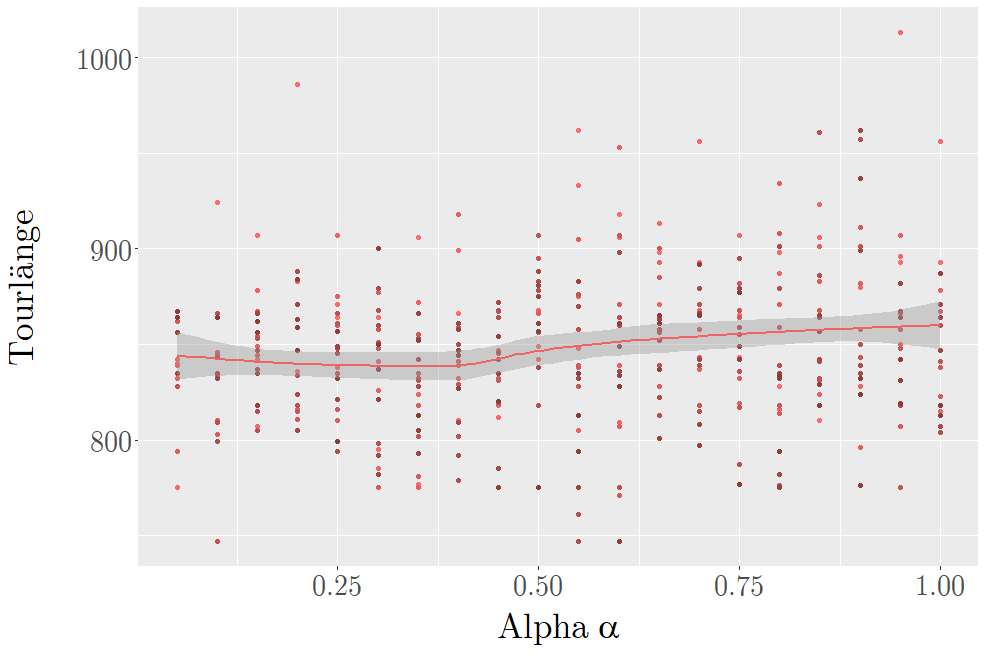
\includegraphics[width=\textwidth]{images/diagramiterativealpha}
            \caption{Alpha $\alpha$}               
            \label{fig:iterativeAlpha}
        \end{subfigure}
        \hfill
        \begin{subfigure}[b]{0.475\textwidth}  
            \centering 
            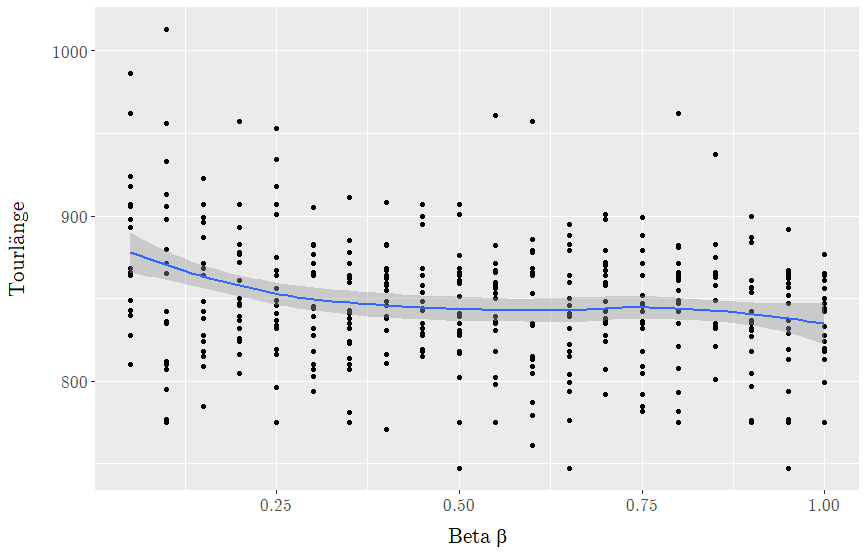
\includegraphics[width=\textwidth]{images/diagramiterativebeta}
            \caption{Beta $\beta$}   
            \label{fig:iterativeBeta}
        \end{subfigure}
        \vskip\baselineskip
        \begin{subfigure}[b]{0.475\textwidth}   
            \centering 
            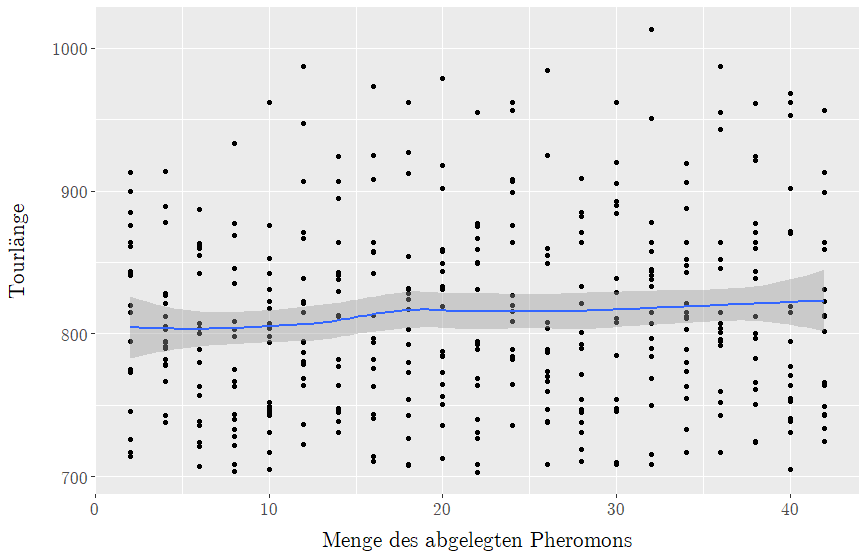
\includegraphics[width=\textwidth]{images/diagramiterativedeposit}
            \caption{Menge des abgelegten Pheromons}   
            \label{fig:iterativeDeposit}
        \end{subfigure}
        \quad
        \begin{subfigure}[b]{0.475\textwidth}   
            \centering 
            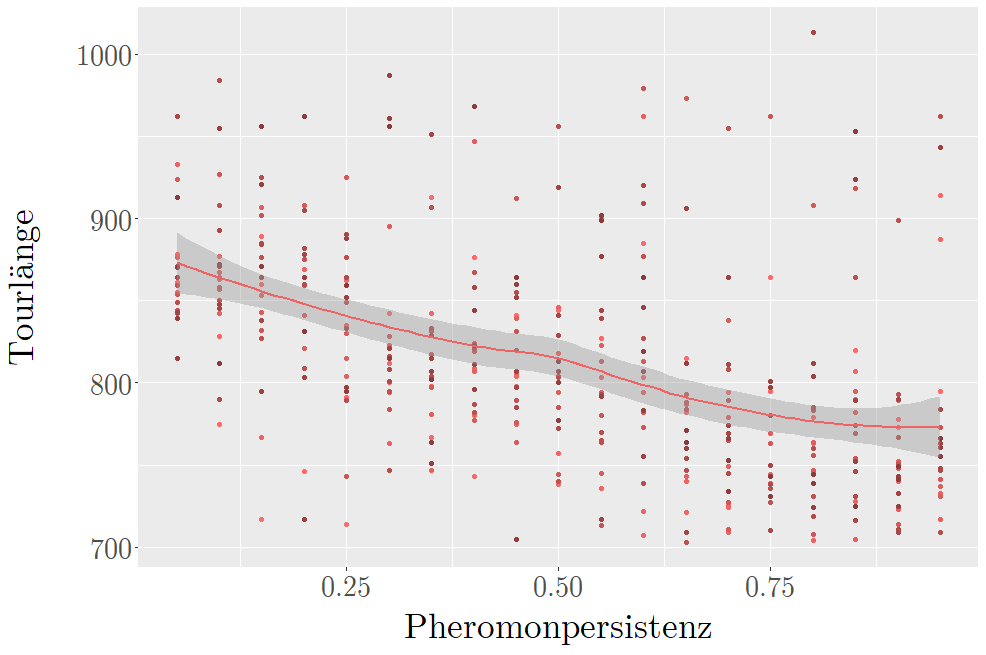
\includegraphics[width=\textwidth]{images/diagramiterativereduction}
            \caption{Pheromonpersistenz}   
            \label{fig:iterativeReduction}
        \end{subfigure}
        \caption{Abhängigkeit der Tourlänge von den einzelnen Parametern bei der iterativen Tourkonstruktion } 
        \label{fig:iterativeDiagram}
    \end{figure}
\subsubsection{Parametereinfluss auf den iterativen Algorithmus mit eingeschränkter Pheromonaktualisierung}
Wie bei dem oben untersuchten iterativen Algorithmus wurden auch hier die Parameter Alpha $\alpha$ und Beta $\beta$ sowie $Q$ und $\rho$ kombiniert untersucht. Dazu wurden wie schon oben gezeigt jeweils eine doppelte \texttt{For}-Schleife verwendet. Aufgrund der höheren Komplexität und damit der höheren Laufzeit wurden die Schrittweiten zwischen den einzelnen Werten doppelt so groß gewählt. Der Wertebereich für die einzelnen Parameter ist für Alpha $\alpha$ und Beta $\beta$ derselbe; für die Pheromonablagemenge wurde eine Wertebereich von $2 \leq Q \leq$, für die Pheromonpersistenz eine Wertebereich von $0,1 \leq \rho \leq 1$ gewählt.
\\Auch wenn dieser Algorithmus vom Namen her auf eine ähnliche Tourlängenbeeinflussung durch die einzelnen Parameter wie der iterative Algorithmus ohne eingeschränkte Pheromonaktualisierung schließen lässt, gestaltet sich diese wesentlich anders. Dies geht aus Abbildung \ref{fig:mmasDiagram} hervor. Der Parameter Beta $\beta$, der die Wichtigkeit der Distanz bei der Ermittlung der nächsten Stadt während der Tourkonstruktion angibt, 
lässt das Finden leicht kürzerer Routen bei Annäherung gegen $1$ zu. Der Parameter Alpha $\alpha$ dagegen beeinflusst das Finden kurzer Touren bei Annäherung gegen $1$ eher negativ. Jedoch ist die Streuung bei kleinen Werten für $\alpha$ wesentlich höher. \\Über den Einfluss der Menge des abgelegten Pheromons lässt sich bei diesem Algorithmus sagen, dass diese ab circa ab einem Wert von $10$ die besten Werte mit einer sehr geringen Streuung erzielt. Für einen Wert von $Q = 2$ erreicht der Algorithmus teilweise Tourlängen mit einer Abweichung von fast $300 \%$ vom Optimum. Die Pheromonpersistenz $\rho$ steigt für höhere Werte leicht an und ist für einen Wert im Bereich von $0,05$ bis $0,10$ optimal im Hinblick auf die Tourlänge sowie vor allem auf eine geringe Streuung.
\begin{figure}
        \centering
        \captionsetup[subfigure]{oneside,margin={0.5cm,0cm}}
        \begin{subfigure}[b]{0.475\textwidth}
            \centering
            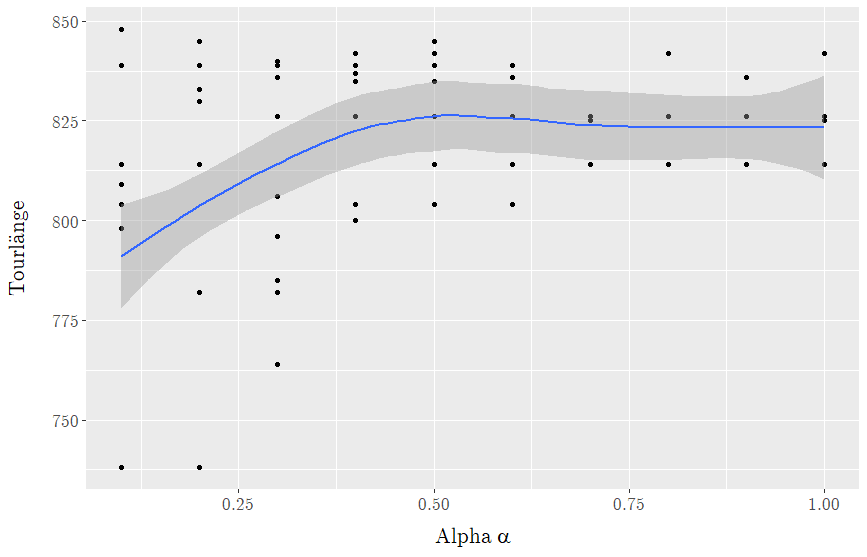
\includegraphics[width=\textwidth]{images/diagrammmasalpha}
            \caption{Alpha $\alpha$}               
            \label{fig:iterativeAlpha}
        \end{subfigure}
        \hfill
        \begin{subfigure}[b]{0.475\textwidth}  
            \centering 
            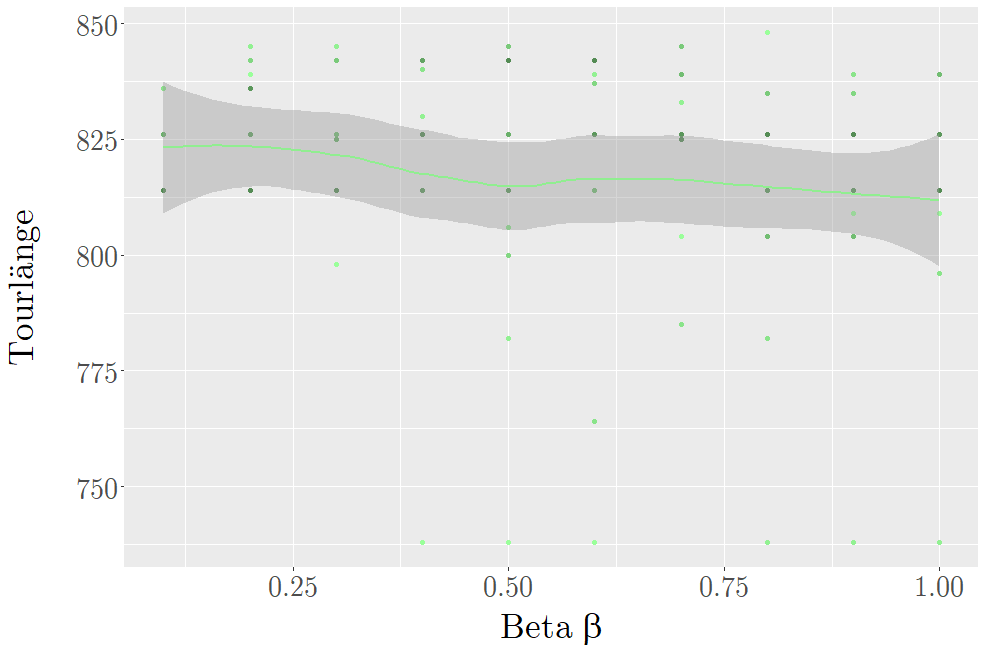
\includegraphics[width=\textwidth]{images/diagrammmasbeta}
            \caption{Beta $\beta$}   
            \label{fig:iterativeBeta}
        \end{subfigure}
        \vskip\baselineskip
        \begin{subfigure}[b]{0.475\textwidth}   
            \centering 
            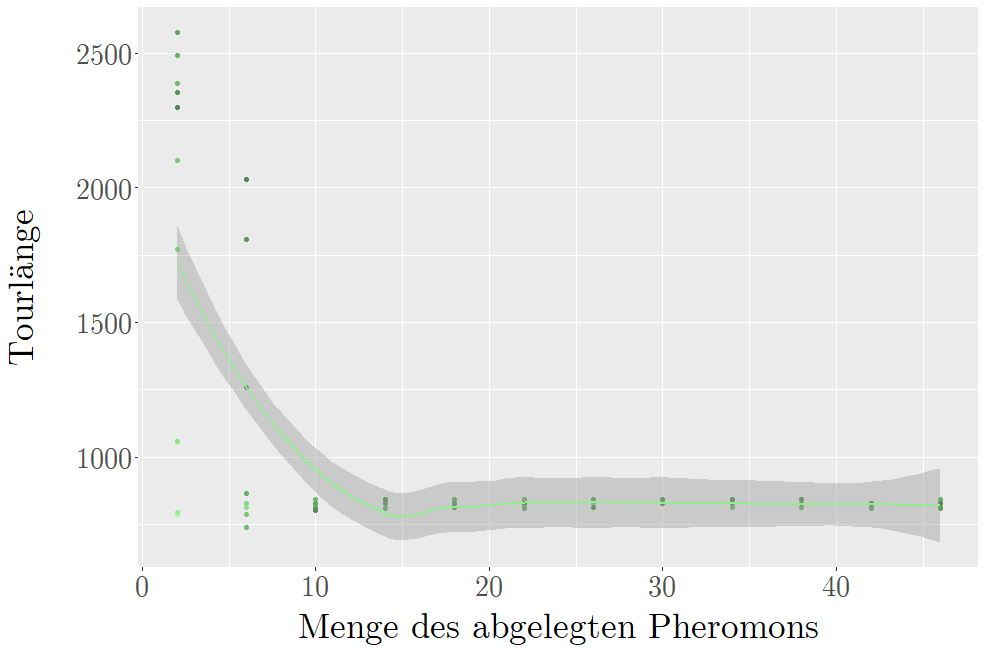
\includegraphics[width=\textwidth]{images/diagrammmasdeposit}
            \caption{Menge des abgelegten Pheromons}   
            \label{fig:iterativeDeposit}
        \end{subfigure}
        \quad
        \begin{subfigure}[b]{0.475\textwidth}   
            \centering 
            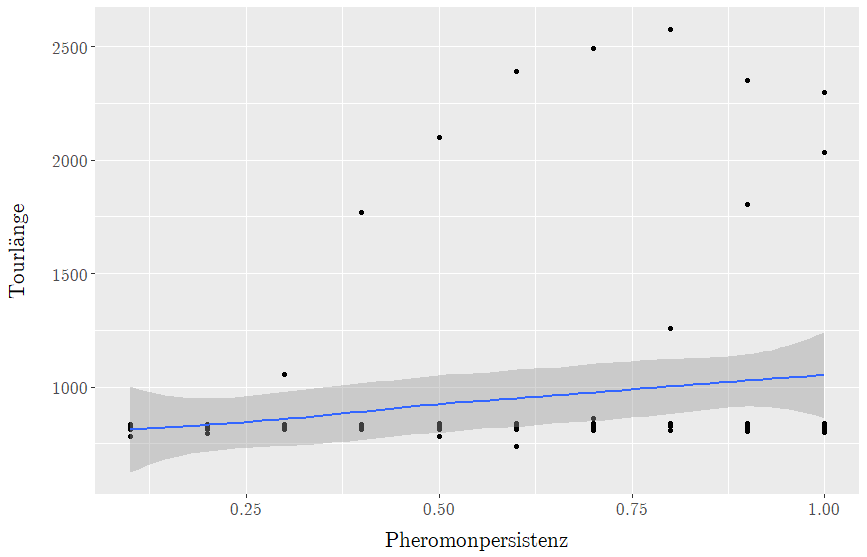
\includegraphics[width=\textwidth]{images/diagrammmasreduction}
            \caption{Pheromonpersistenz}   
            \label{fig:iterativeReduction}
        \end{subfigure}
        \caption{Abhängigkeit der Tourlänge von den einzelnen Parametern bei der iterativen Tourkonstruktion mit eingeschränkter Pheromonaktualisierung } 
        \label{fig:mmasDiagram}
    \end{figure}
\subsubsection{Parametereinfluss auf den parallelen Algorithmus}
Beim dritten und letzten implementierten Algorithmus wird der Parametereinfluss wie bei den zwei vorhergehenden Algorithmen auch durch Kombination der Parameter untersucht. Auch hier wird Alpha $\alpha$ und Beta $\beta$ zusammen im Intervall von $0,05 \leq \{\alpha,\beta\} \leq 1$ untersucht - jeweils mit einer Schrittweite von $0,05$. Anhand von Abbildung \ref{fig:parallelDiagram} lässt sich erkennen, dass für Alpha $\alpha$ bessere Tourlängenwerte bei Annäherung gegen $1$ erzielt werden. Für Beta $\beta$ ist dieser Sachverhalt genau umgekehrt - hier werden die besten Werte bei einem geringen Einfluss der Distanz auf die Tourkonstruktion erzielt.\\Für die Pheromonablage- und Pheromonpersistenzwerte werde wurde ein Wertebereich von $2 \leq Q \leq 42$ bzw. $0,05 \leq \rho \leq 0,95$ gewählt. Für diese Parameter lässt sich keine große Veränderung der Tourlängen feststellen; die gefundenen Tourlängen sind im Mittel konstant für alle unterschiedlichen Werte.
\begin{figure}
        \centering
        \captionsetup[subfigure]{oneside,margin={0.5cm,0cm}}
        \begin{subfigure}[b]{0.475\textwidth}
            \centering
            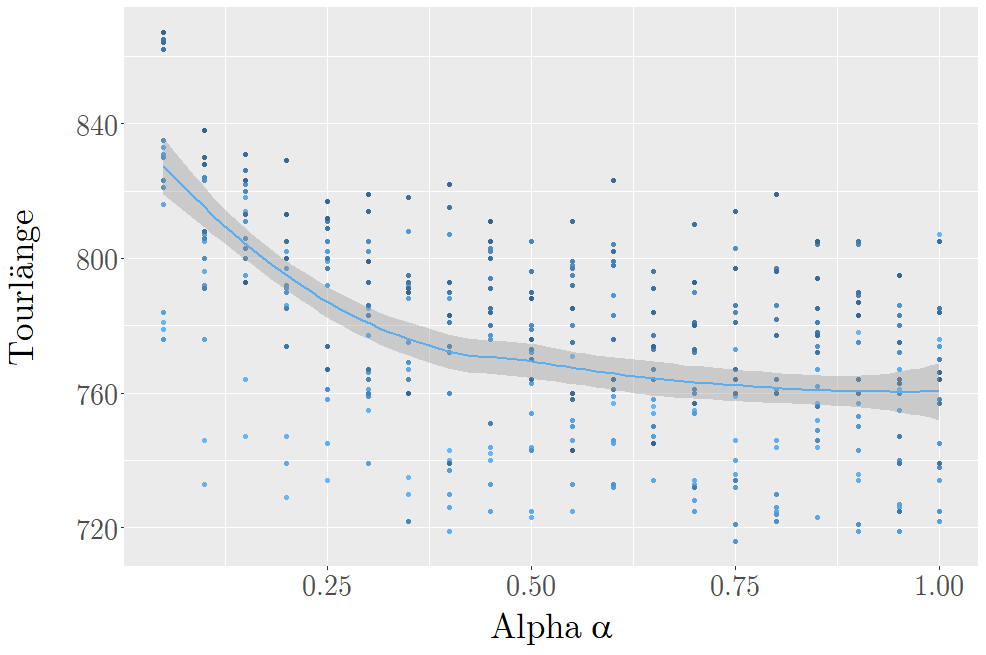
\includegraphics[width=\textwidth]{images/diagramparallelalpha}
            \caption{Alpha $\alpha$}               
            \label{fig:iterativeAlpha}
        \end{subfigure}
        \hfill
        \begin{subfigure}[b]{0.475\textwidth}  
            \centering 
            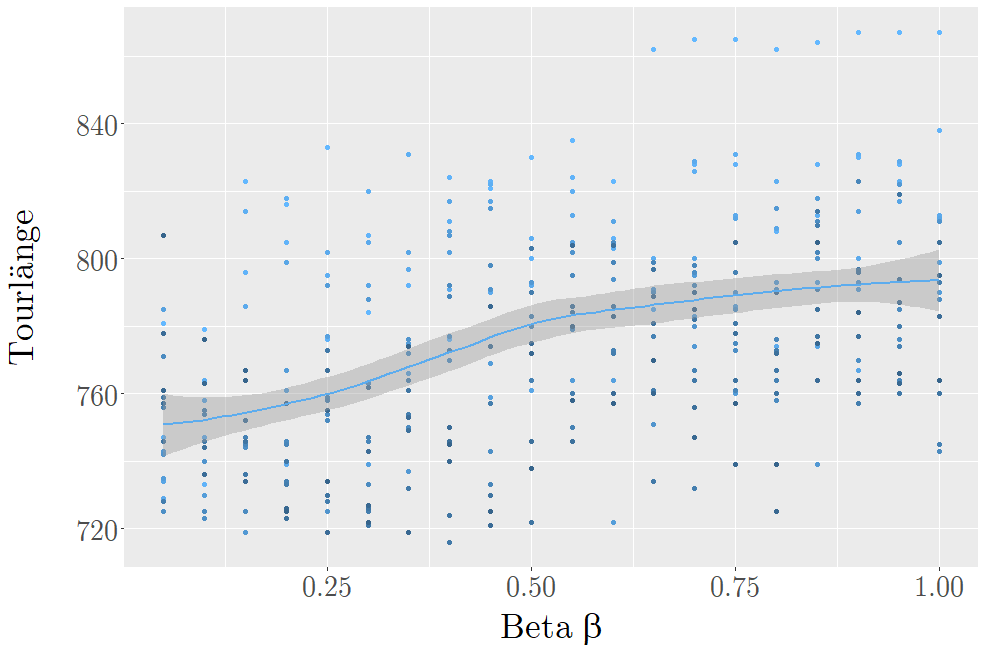
\includegraphics[width=\textwidth]{images/diagramparallelbeta}
            \caption{Beta $\beta$}   
            \label{fig:iterativeBeta}
        \end{subfigure}
        \vskip\baselineskip
        \begin{subfigure}[b]{0.475\textwidth}   
            \centering 
            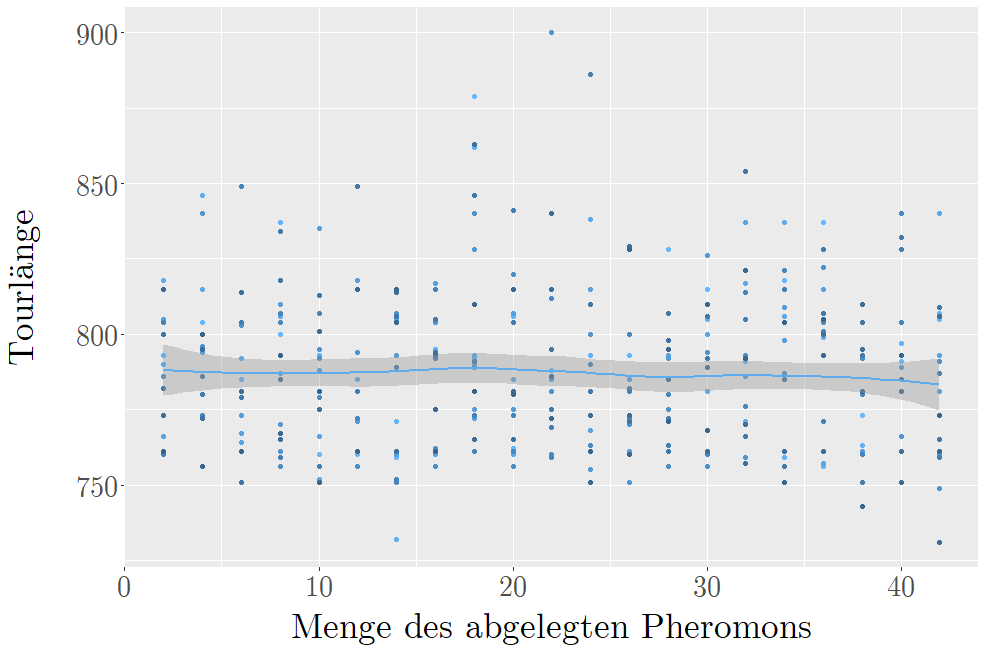
\includegraphics[width=\textwidth]{images/diagramparalleldeposit}
            \caption{Menge des abgelegten Pheromons}   
            \label{fig:iterativeDeposit}
        \end{subfigure}
        \quad
        \begin{subfigure}[b]{0.475\textwidth}   
            \centering 
            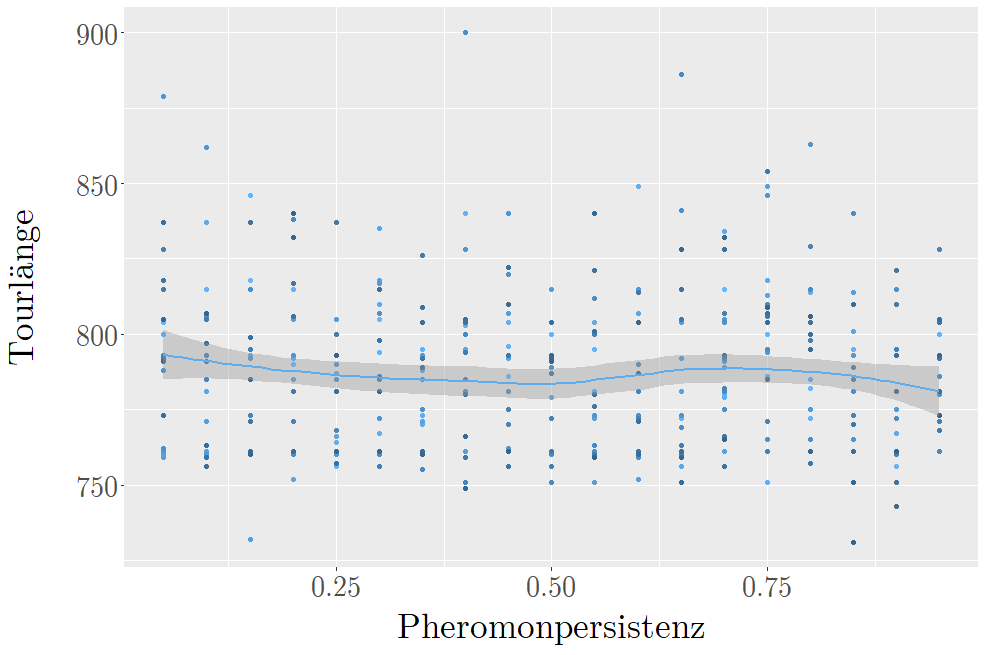
\includegraphics[width=\textwidth]{images/diagramparallelreduction}
            \caption{Pheromonpersistenz}   
            \label{fig:iterativeReduction}
        \end{subfigure}
        \caption{Abhängigkeit der Tourlänge von den einzelnen Parametern bei der parallelen Tourkonstruktion } 
        \label{fig:parallelDiagram}
    \end{figure}
\subsection{Auswirkung des gewählten Wahrscheinlichkeitsalgorithmus}
Wie schon in Abschnitt \ref{enum:Update} vorgestellt, wurden für die Erstellung dieser Arbeit zwei verschiedene Algorithmen zur Ermittlung der Wahrscheinlichkeiten der nächsten Städte bei der Tourkonstruktion implementiert. Diesen Algorithmen liegt zum einen die Formel \ref{eq:Prob} zugrunde, die auch von Thomas Stützle und Holger H. Hoos in ihrem vorgestellten \textit{MAX-MIN Ant System} verwendet wurde. Im folgenden wird der Algorithmus, der diese Formel verwendet, der Einfachheit halber \textit{Komplexer Wahrscheinlichkeitsalgorithmus} genannt. Der andere Algorithmus verwendet eine stark vereinfachte Form dieser Formel (Gleichung \ref{eq:ProbSimple}) und wird im folgenden als \textit{Einfacher Wahrscheinlichkeitsalgorithmus} bezeichnet.
\\Bei der Untersuchung wurden für die einzelnen Parameter folgende empirische Werte verwendet: $\alpha = 1$, $\beta = 0,25$, $Q = 40$ und $\rho = 0,15$. Für die Erhebung von statischen Daten wurde jeder Algorithmus zur Tourkonstruktion mit jedem Wahrscheinlichkeitsalgorithmus zehnmal getestet. Die verwendete Probleminstanz war \texttt{dantzig42} mit einem Tourlängenoptimum von $699$.
\\\\Die Ergebnisse sind in folgender Tabelle dargestellt:
\begin{table}[]
\captionsetup{justification=centering}
\centering
\resizebox{\textwidth}{!}{%
\begin{tabular}{@{}lllllll@{}}
\toprule
 & \multicolumn{6}{c}{Wahrscheinlichkeitsermittlung} \\
 & \multicolumn{3}{c|}{Einfach} & \multicolumn{3}{c}{Komplex} \\
\multicolumn{1}{c|}{Algorithmus} & \begin{tabular}[c]{@{}l@{}}Tourlänge\\ (Durchschnitt)\end{tabular} & {[}\%{]} & \multicolumn{1}{l|}{Zeit in $s$} & \begin{tabular}[c]{@{}l@{}}Tourlänge\\ (Durchschnitt)\end{tabular} & {[}\%{]} & Zeit in $s$ \\ \midrule
\multicolumn{1}{l|}{Iterativ} & 746,3 & 6,77 & \multicolumn{1}{l|}{3,49} & 733,1 & 4,88 & 55,46 \\
\multicolumn{1}{l|}{Iterativ mit eingeschränkter Pheromonaktualisierung} & 849,7 & 21,56 & \multicolumn{1}{l|}{5,13} & 880,5 & 25,97 & 71,23 \\
\multicolumn{1}{l|}{Parallel} & 818 & 17,02 & \multicolumn{1}{l|}{23,33} & 832,6 & 19,11 & 447,45 \\ \bottomrule
\multicolumn{7}{l}{}
\end{tabular}%
}
\caption{Ergebnisse für die einzelnen in Algorithmen in Abhängigkeit von dem gewählten Wahrscheinlichkeitsalgorithmus. Die Prozentzahl hinter der Tourlänge zeigt die Abweichung vom Tourlängenoptimum $d = 699$ an}
\label{table:Prob}
\end{table}
\\Auffallend ist zu aller erst, dass der komplexe Wahrscheinlichkeitsalgorithmus im Vergleich zu dem einfachen Algorithmus sehr viel mehr Zeit zur Berechnung benötigt. Dieser Unterschied beträgt teilweise bis zu $2000 \,\%$.
Im Hinblick auf die gefundenen Routenlängen lässt  sich kein großer Unterschied feststellen. Bei dem Iterativen Algorithmus mit eingeschränkter Pheromonaktualisierung und der parallelen Tourkonstruktion sind die durchschnittlichen Routenlängen bei Benutzung des einfachen Wahrscheinlichkeitsalgorithmus sogar kleiner.
\subsection{Ergebnisse der Algorithmen bei verschiedenen TSP-Probleminstanzen}
Abschließend werden nun die drei implementierten Tourkonstruktionsalgorithmen auf vier verschiedenen TSP-Probleminstanzen angewendet, die der \texttt{TSPLIB95} entnommen wurden. Gewählt wurden die Instanzen \texttt{burma14}, \texttt{dantzig42}, \texttt{gr120} und \texttt{si535}. Für alle Algorithmen wurde der eigene, einfache Wahrscheinlichkeitsalgorithmus verwendet.
\\In der untenstehenden Tabelle \ref{table1} sind die Ergebnisse und die jeweiligen verwendeten Werte für die verschiedenen Parameter aufgelistet.
\\Die Probleminstanz \texttt{si535} wurde aufgrund der absehbar hohen Laufzeit nicht mit dem \textit{Iterativen Algorithmus mit eingeschränkter Pheromonaktualisierung} untersucht. Die Angabe der Laufzeit ist in dem Fall ein geschätzter Wert, der durch den Vergleich mit anderen Laufzeiten zustande kommt.
\\Für die beiden iterativen Algorithmen wurden unterschiedliche Werte der Parameter abhängig von der Anzahl der Städte einen Problems verwendet. Diese Vorgehensweise resultiert resultiert aus einem besseren Ergebnis im Hinblick auf die Effektivität. Dabei sind sowohl die einzelnen Parameterwerte als auch die Städtezahl, bei sich diese Parameter ändern, empirisch bestimmte Werte die unter anderem auf den Ergebnissen von Abschnitt \ref{sec:einflussparameter} basieren.
\\Die Auswertung der Ergebnisse folgt im nächsten Abschnitt dieser Arbeit. Grob gesehen lässt sich aber erkennen, dass der iterative Algorithmus die besten Werte erzielt während der Iterative Algorithmus mit eingeschränkter Pheromonaktualisierung am schlechtesten abschneidet; auch was die Laufzeit des Algorithmus betrifft.
\newpage
\begin{landscape}
\begin{table}[]
\centering
\resizebox{\columnwidth}{!}{%
\begin{tabular}{@{}llllllllllll@{}}
\toprule
          &         &                                            & \multicolumn{6}{c}{gefundene Routen}                                                   & \multicolumn{3}{c}{Laufzeiten in Sekunden}             \\
Name      & Optimum & \multicolumn{1}{l|}{Algorithmus}           & Minimum & {[}\%{]} & Maximum & {[}\%{]} & Durchschnitt & \multicolumn{1}{l|}{{[}\%{]}} & Minimum          & Maximum          & Durchschnitt     \\ \midrule
burma14   & 3323    & \multicolumn{1}{l|}{Iterativ}              & 3336    & 0,3      & 3803    & 14,4     & 3450,2       & \multicolumn{1}{l|}{3,8}      & 0,53             & 0,54             & 0,53             \\
                 &         & \multicolumn{1}{l|}{Iterativ mit eing. PA} & 3381    & 1,7      & 3381    & 1,7      & 3381         & \multicolumn{1}{l|}{1,7}      & 3,34             & 3,38             & 3,31             \\ 
 &         & \multicolumn{1}{l|}{Parallel}              & 3323    & 0        & 3323    & 0        & 3323         & \multicolumn{1}{l|}{0}        & 0,50             & 0,55             & 0,52             \\ \midrule
dantzig42 & 699     & \multicolumn{1}{l|}{Iterativ}              & 704     & 0,7      & 755     & 8        & 721,9        & \multicolumn{1}{l|}{3,2}      & 4,32             & 5,84             & 5,51             \\
&         & \multicolumn{1}{l|}{Iterativ mit eing. PA} & 814     & 16,4     & 836     & 19,6     & 824,2        & \multicolumn{1}{l|}{17,9}     & 22,74            & 23,59            & 23,01            \\
          &         & \multicolumn{1}{l|}{Parallel}              & 731     & 4,6      & 764     & 9,3      & 749,3        & \multicolumn{1}{l|}{7,2}      & 3,34             & 3,39             & 3,37             \\  \midrule
gr120     & 6942    & \multicolumn{1}{l|}{Iterativ}              & 8166    & 17,63    & 8286    & 19,3     & 8221,6       & \multicolumn{1}{l|}{18,4}     & 32,22            & 44,45            & 42,77            \\       
          &         & \multicolumn{1}{l|}{Iterativ mit eing. PA} & 8322    & 27,2     & 8832    & 27,2     & 8832         & \multicolumn{1}{l|}{27,2}     & 173,53           & 202,95           & 182,84           \\ 
   &         & \multicolumn{1}{l|}{Parallel}              & 8198    & 18,1     & 8778    & 26,4     & 8540,2       & \multicolumn{1}{l|}{21,7}     & 24,02            & 26,08            & 24,64            \\\midrule
si535     & 48450   & \multicolumn{1}{l|}{Iterativ}              & 50101   & 3,4      & 53532   & 10,4     & 51529,3      & \multicolumn{1}{l|}{6,35}     & 657,10           & 687,36           & 673,59           \\
    &         & \multicolumn{1}{l|}{Iterativ mit eing. PA} & -       & -        & -       & -        & -            & \multicolumn{1}{l|}{-}        & ($\sim$1 Stunde) & ($\sim$1 Stunde) & ($\sim$1 Stunde) \\
          &         & \multicolumn{1}{l|}{Parallel}              & 70438   & 45,3     & 74246   & 53,2     & 72137,8      & \multicolumn{1}{l|}{48,89}    & 466,01           & 570,11           & 503,40           \\  \bottomrule
\end{tabular}%
}
\resizebox{\columnwidth}{!}{%
\begin{tabular}{ll|llllll}
\multicolumn{8}{l}{}  \\
\multicolumn{8}{l}{}  \\ 
\multicolumn{8}{l}{}  \\ 
\multicolumn{8}{l}{}  \\
\multicolumn{8}{l}{}  \\
\multicolumn{8}{l}{}  \\
\multicolumn{8}{l}{}  \\ 
\multicolumn{8}{l}{}  \\ \toprule
Algorithmus           &                      & Alpha $\alpha$ & Beta $\beta$ & Pheromonablagemenge $Q$ & Pheromonpersistenz $\rho$ & Anzahl an Ameisen & \multicolumn{1}{c}{\begin{tabular}[c]{@{}c@{}}Iterationen\\ bzw. Iterationsschwelle\end{tabular}} \\ \hline
Iterativ              & $|V| \textless{}=$ 100 & 1     & 0,25 & 40                    & 0,15                      & 1000              & 500                                                                                               \\
                      & $|V| \textgreater 100$ & 0,1   & 0,9  & 10                    & 0,9                       & 1000              & 500                                                                                               \\ \hline
Iterativ mit eing. PA & $|V| \textless{}= 100$ & 1     & 0,25 & 10                    & 0,15                      & 500               & 8                                                                                                 \\
                      & $|V| \textgreater 100$ & 0,1   & 0,9  & 10                    & 0,05                      & 500               & 8                                                                                                 \\ \hline
Parallel              &                      & 1     & 0,1  & 42                    & 0,15                      & 500               & -                                                                                                 \\ \bottomrule
\multicolumn{8}{l}{}  \\ 
\end{tabular}%
}
\\\caption{Gefundene Touren von Probleminstanzen aus der \texttt{TSPLIB95} in Abhängigkeit von dem gewählten Algorithmus. Der \textit{Iterative Algorithmus mit eingeschränkter Pheromonaktualisierung} wird in dieser Tabelle mit \glqq Iterativ mit eing. PA\grqq{} abgekürzt. Die Zahl in dem Namen der Probleminstanz gibt die Anzahl der Städte in dieser an. Weiterhin stehen die Prozentangaben hinter den Tourlängen für die Abweichung vom jeweiligen Optimum. Die untere Tabelle gibt Auskunft über die verwendeten Parameter beim Versuchsdurchlauf. Um statistisch verwertbare Daten zu erhalten wurde jeder Versuch zehnmal durchgeführt.}
\label{table1}
\end{table}
\end{landscape}
\section{Auswertung und Vergleich}
\subsection{Vergleich der iterativen und parallelen Implementierung}
\subsection{Vergleich mit der optimalen Lösung}
\subsection{Vergleich mit der Laufzeit und Komplexität von anderen Algorithmen}
\section{Zusammenfassung und Fazit}
\newpage
\appendix
\section{Erklärung der implementierten grafischen Oberfläche}
\begin{figure}
\captionsetup{justification=centering}
  \centering
     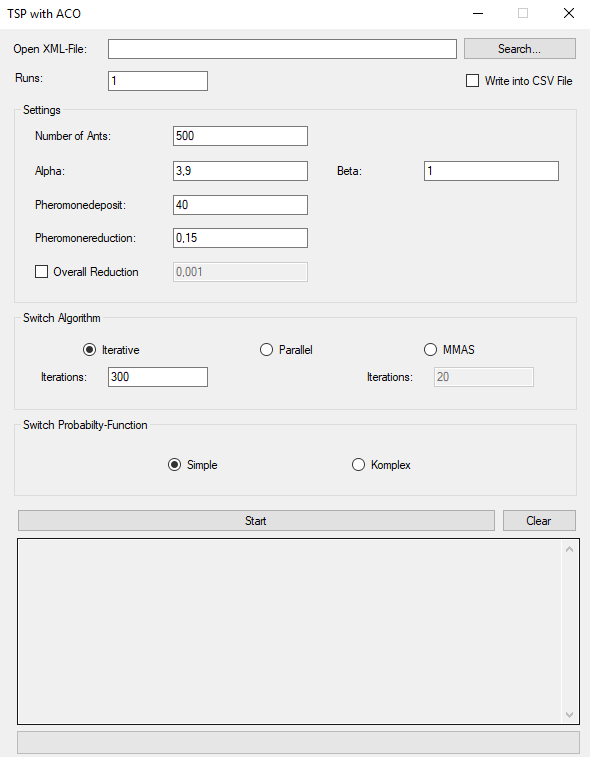
\includegraphics[width=0.7\textwidth]{images/TSPACOGUI.png}
  \caption{Grafische Oberfläche des Programms}
  \label{img:gui}
\end{figure}
Der Button \textbf{Search...} öffnet einen neuen Filedialog, mit dem die gewünschte Probleminstanz im XML-Format geladen werden kann. Alternativ kann der Dateipfad auch in das nebenstehende Textfeld eingegeben werden.
\\\\Der Paramater im Textfeld \textbf{Runs} gibt an, wie oft das gesamte Programm ausgeführt werden soll. Dies ist hilfreich bei der Ermittlung von Durchschnittswerten für einzelne festgelegte Parameter.
\\\\Unter \textbf{Settings} befinden sich alle konfigurierbaren Parameter, die Einfluss auf den Algorithmus haben. 
\\\textbf{Number of Ants} gibt die Anzahl der Ameisen an, welche die Route konstruieren. \textbf{Alpha} steht für die Wichtigkeit der Pheromonspur, \textbf{Beta} für die Wichtigkeit der Distanz bei der Ermittlung der nächsten Stadt im Verlauf der Tourkonstruktion. Der Parameter \textbf{Pheromondeposit} gibt die Menge des ablegten Pheromons an, während \textbf{Pheromonereduction} für die Verdunstungsmenge steht.
\\\\Unter \textbf{Switch Algorithm} kann der gewünschte Algorithmus zur Berechnung der kürzesten Route gewählt werden. \textbf{Iterations} gibt dabei für den iterativen Algorithmus die Anzahl von Iterationen an, nach denen der Algorithmus abbricht, wenn keine kürzere Route gefunden wurde. Analag gibt er für die Option \textbf{Iterative with restricted Pheromoneupdate} an, wie oft alle Ameisen ihre Tour konstruieren.
\\\\Mit \textbf{Switch Probability-Function} kann zwischen einem einfachen und einem komplexeren Algorithmus zur Ermittlung der nächsten jeweiligen Stadt bei der Erstellung der Route ausgewählt werden.
\\\\Ein Klick auf den Button \textbf{Start} startet den Algorithmus. Die Ausgabe erfolgt in das untenstehende Textfeld, welches mit dem Button \textbf{Clear} geleert werden kann.
\\\\Möchte man zudem eine Ausgabe in eine Tabellendatei erhalten, muss oben rechts die Funktion \textbf{Write into CSV File} aktiviert werden.
\newpage
\section{Hinweise zur Nutzung des Programms als Konsolenapplikation}
Die Implementierung des Ameisenalgorithmus zur Lösung von TSP-Probleminstanzen kann auch auf Konsolenbasis unter Windows genutzt werden. Hierbei wird der Pfad und die einzelnen Optionen als Runtime-Parameter übergeben. Insgesamt müssen dabei jeweils 13 Parameter gesetzt werden.
\begin{enumerate}
\item Dateipfad (Datei muss dabei als \texttt{XML}-Datei vorliegen)
\item Anzahl der Ameisen, die eine Tour generieren
\item Gewünschter Algorithmus: \glqq 0\grqq\, entspricht dem Iterativen Algorithmus, \glqq 1\grqq\, dem parallelen Algorithmus und \glqq 2\grqq\, dem Iterativen Algorithmus mit eingeschränkter Pheromonaktualisierung
\item Wert für die Menge an abgelegtem Pheromon $Q$ - sollte zwischen $0.05$ und $80$ liegen
\item Wert für die Pheromonverdunstung $1 - \rho$ - sollte zwischen $0.01$ und $0.99$ liegen
\item Wert für den Parameter Alpha $\alpha$ - sollte zwischen $0.01$ und $1$ liegen
\item Wert für den Parameter Beta $\beta$ - sollte zwischen $0.01$ und $1$ liegen
\item Schalter für eine optionale allgemeine Reduzierung der Pheromonmatrix nach jeder Tourkonstruktion - für \glqq 0\grqq\, ist die Option deaktiviert, für \glqq 1\grqq\, aktiviert
\item Wert für die optionale allgemeine Reduzierung der Pheromonmatrix - sollte zwischen $0.001$ und $0.1$ liegen
\item Anzahl der Iterationen für den Iterativen Algorithmus, bei der Wahl von anderen Algorithmen \glqq 0\grqq\, eintragen
\item Anzahl der Iterationen beim Iterativen Algorithmus mit eingeschränkter Pheromonaktualisierung, bei der Wahl von anderen Algorithmen \glqq 0\grqq\, eintragen
\item Schalter für den Wahrscheinlichkeitsalgorithmus - bei \glqq 0\grqq\, wird der einfache Algorithmus verwendet, bei \glqq 1\grqq\, der komplexe Algorithmus
\item Schalter für die Ausgabe in eine CSV-Datei - dieser ändert den Output des Programms sodass für eine einfache weitere Verwendung in einem CSV-Datensatz - für \glqq 0\grqq\, ist die Option deaktiviert, für \glqq 1\grqq\, aktiviert
\end{enumerate}
Für die Verwendung des Iterativen Algorithmus mit $1000$ Ameisen und einer Iterationsschwelle von $500$ zur Lösung der \texttt{burma14}-Probleminstanz könnte der Prozessaufruf so aussehen:
\begin{lstlisting}
TSPACO.exe burma14.xml 1000 1 40.0 0.14 1.0 0.25 0 0.001 500 0 0 0
\end{lstlisting}

\newpage
\bibliography{literatur}{}
\addcontentsline{toc}{section}{Literatur} 
\end{document}